\graphicspath{{graphics/}}

\chapter{Trajectory Planning}
\label{cha:trajectory}
For the two most advanced modes, i. e. the Half-Automatic and the Full-Automatic Mode, trajectories had to be generated. In this chapter the best trajectories for \textsc{Skye} are elaborated and tested with suitable trajectory controllers. Performance results based on a \textsc{Matlab} simulation are shown.

%\subsection{Our Approach}
%From the GUI it was given that the goal trajectory would be a multipoint-interpolating %trajectory. The user is able to define waypoints on a map which afterwards should be %connected with a reasonable and realizable trajectory. Beside interpolating trajectories %there exist also approximating trajectories but they were not taken into consideration, since %usually the user wants skye fly directly through a waypoint.

%In another Bsc Thesis elaborated in this project a controller for waypoint following was %designed. So it was convenient in the scope of this Thesis to use this controller instead of %a specialized trajectory controller.

\section{Experimental Design}
The main application fields of the system \textsc{Skye} are image capturing and agile performance demonstrations. The waypoints used to test the trajectory algorithms had therefore to be alike these situations. All the results below belong to the three sample waypoints shown in figure \ref{fig:sampleNodes}. Indeed, to verify the conclusions, some more situations had to be considered.

\begin{figure}[h]
  \begin{minipage}[t]{0.32\textwidth}
    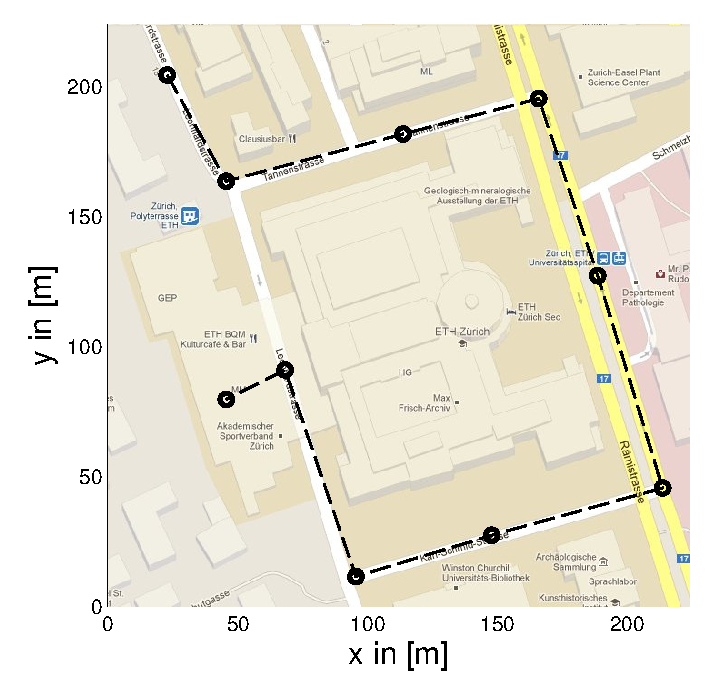
\includegraphics[width = \textwidth]{graphics/sampleNodeRoad}
  \end{minipage}
  \hfill
  \begin{minipage}[t]{0.32\textwidth}
    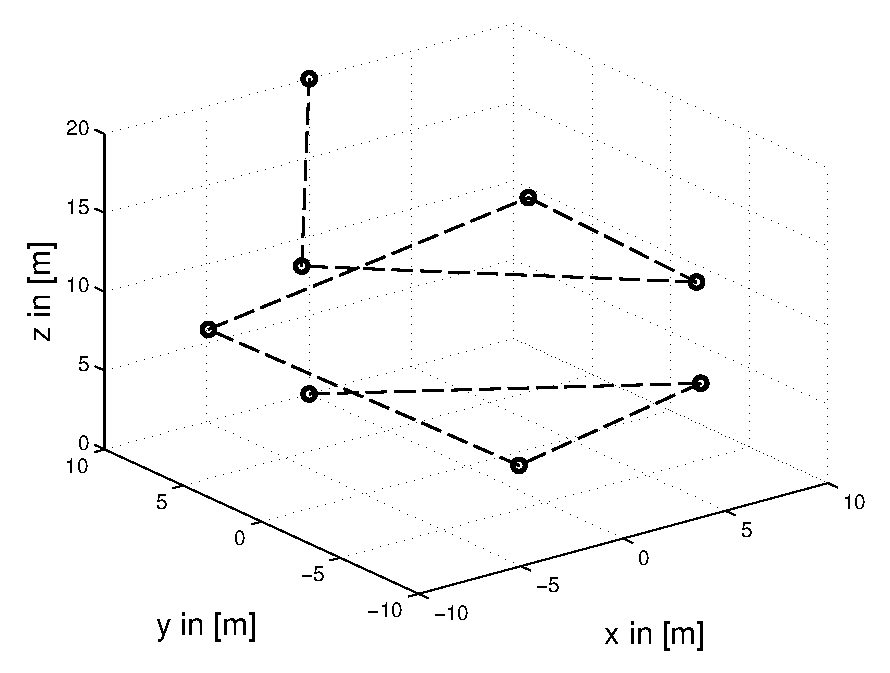
\includegraphics[width = \textwidth]{graphics/sampleNodeHelix}
  \end{minipage}
  \hfill
  \begin{minipage}[t]{0.32\textwidth}
    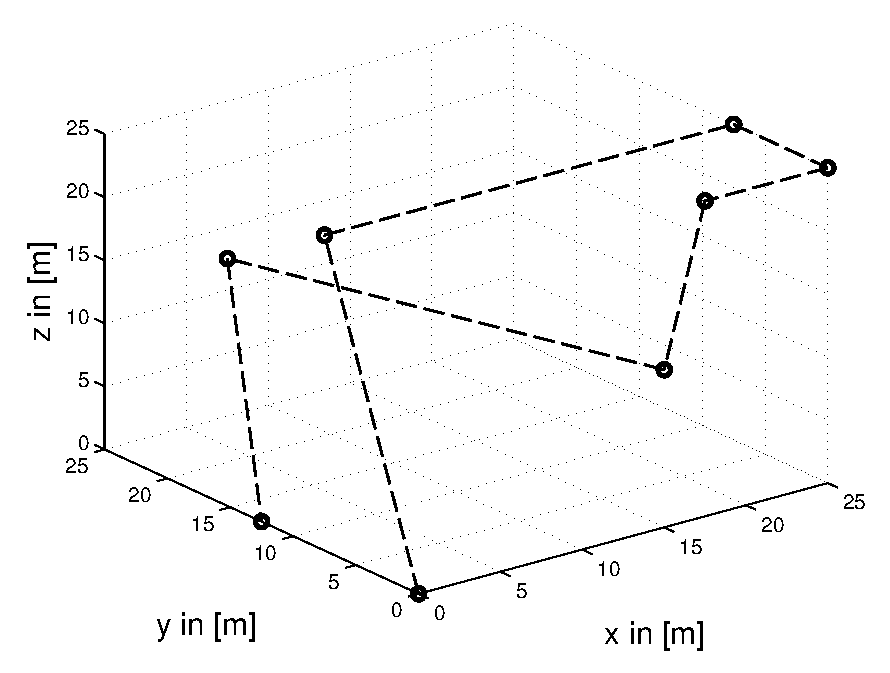
\includegraphics[width = \textwidth]{graphics/sampleNodeAgile}
  \end{minipage}
  \caption{The experimental environment based on three samples. The \textit{road} waypoints (left) represent the need of low overshoots to not touch obstacles beside the streets. Its long straight ways enable high velocities. The \textit{helix} waypoints represents the circumnavigation of any obstacle. It yields to high curvatures of the track. The \textit{agile} waypoints include both straight sections as high curvatures.}
  \label{fig:sampleNodes}
\end{figure}

\begin{figure}
\centering
\def\svgwidth{\columnwidth}
\input{graphics/drawing.pdf_tex}
\end{figure}


Furthermore, to score (\textbf{and optimize?}) the generated trajectories $\tilde{p}(t)$ and the resulting trace of the system $r(t)$, we set up the following criteria. Criteria (\ref{item:static_deviation}) to (\ref{item:static_acceleration}) are refered to as \textit{static criteria} as they do not depend any simulation. The remaining ones (\textit{dynamic criteria}) then mainly depend on the used controller.
\begin{enumerate}[i)]

\item DEVIATION BETWEEN CHORD CONNECTION AND PATH
\label{item:static_deviation}
\item CURVATURES OF PATH
\label{item:static_curvature}
\item ACELLERATION OF TRAJECT
\label{item:static_acceleration}
\item DEVIATION BET TRAJ AND TRACE
\label{item:dynamic_deviation}
\item ACCELERATION OF TRACE
\label{item:dynamic_acceleration}
\item TIME SYNCHRONITY
\label{item:dynamic_synchronity}

\end{enumerate}


\section{Definition of Trajectories}
\label{sec:definition}
\subsection{Paths and Trajectories}

\begin{figure}[h]
\centering
\def\svgwidth{0.9\textwidth}
\input{graphics/PathTrajectory.pdf_tex}
\end{figure}



\subsection{Interpolation and Approximation}
If one wants to draw a curve through a set of data points, there exists two ways to do this. First, the curve can pass through all data points no matter how many bends it will have, secondly, the curve tries to best fit the data, i.e. a function of a  certain order is adopted to best fit the date. This can be done with different methods, e.g with least-squares. Depending on the choice, different curves with different properties are formed (see figure \ref{fig:ApproxInterpol}).  


\begin{figure}[h]
  \begin{minipage}[t]{0.9\textwidth}
    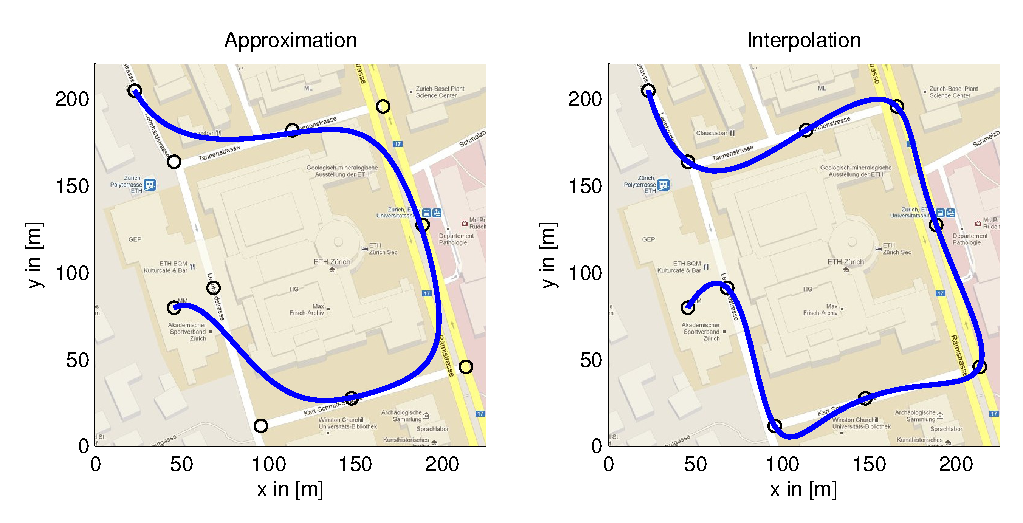
\includegraphics[width = \textwidth]{graphics/ApproxInterpol.eps}
  \end{minipage}
  \hfill
  \begin{minipage}[t]{0.8\textwidth}
%    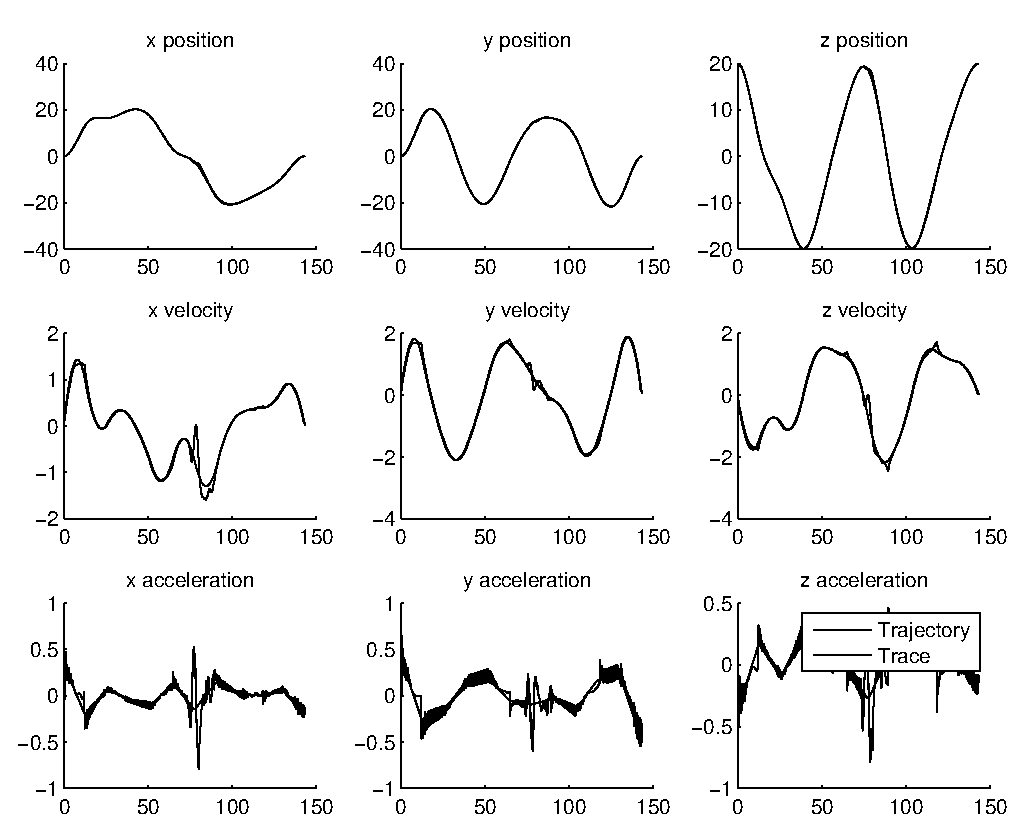
\includegraphics[width = \textwidth]{graphics/b.eps}
  \end{minipage}
  \caption{Interpolation and approximation of waypoints}
  \label{fig:ApproxInterpol}
\end{figure}

If the pilot  defines the trajectory with a set of waypoints, i.e. data points, he usually wants the UAV to pass through all of them. Therefore the waypoints must be interpolated and not approximated with a suitable curve. Instead of using polynomials of degree BLA BLA, splines were chosen.


\section{Spline Theory}
A set of data points can be interpolated with one single curve or with a set of curves defined over a certain interval.  For a 
\label{sec:splineTheory}
references to \cite{engeln}, \cite{biagiotti} and \cite{doessegger}
\subsubsection{Continuity}
\subsubsection{Boundary Conditions}
\subsubsection{Polynomial Order}
\subsubsection{Parametrization}
\subsection{Piecewise Polynomial Interpolating Splines}
\subsubsection{Boundary Conditions}
\subsubsection{Polynomial Order}
\subsubsection{Parameterization}
\subsection{B-Splines}
\subsubsection{Boundary Conditions}
\subsubsection{Polynomial Order}
\subsubsection{Parametrization}

\section{Trajectory Generation}
\label{sec:trajectoryGeneration}
\subsection{System Constraints}
\subsubsection{Maximum Velocities and Accelerations}
In order to plan a feasible trajectory one has to know the capabilities of the system. Here just a basic derivation for the velocities and accelerations is given, for more details refer to (!!!!Bsc Thesis Joe, Bsc Thesis Andy)\\

The maximum feasible acceleration in any direction is calculated to be:

\begin{equation}
  \left|a_{max} \right| =  \frac{\left|F_{res, w}\right|}{m_{tot}} = 0.96 m/s^2
\end{equation}

Whereas the $F_{res,w}$ is the force resulting from all four thrusters operated under full load in the worst direction and $m_{tot}$ is the sum of the masses of the helium, the virtual mass and the mass of the system itself.\\


The maximum feasible velocity in any direction is calculated to be:

\begin{equation}
\left|v_{max} \right| = \sqrt{\frac{\left|F_{res,w} \right|}{\frac{1}{2}c_d \rho \pi r^2}}=2.9 m/s
\end{equation}

which is nothing but $ \left|F_{res,min} \right| = \left|F_{dray} \right| $.\\

For trajectories for position and orientation the maximal feasible angular acceleration is also important. It is calculated to be:

\begin{equation}
  \left|\Psi_{max} \right| =  \frac{\left|M_{res,w}\right|}{\left| \lambda_{max, J_{B}} \right|} = 2.06 rad/s^2 
\end{equation}

which is quite conservative because it is assumed that worst axis for turning is also the principle axis of the inertia tensor with the highest inertia.\\

Since the system is almost undamped for rotations, the rotational velocities will never be the limiting factor.

\subsection{Time Parametrization}

\section{Controller Implementation}
Some commonly used trajectory controllers\footnote{\cite{snider} provides a good overview to trajectory control.} are tested to follow the defined trajectories. The \textit{Trajectory following} controller supplies the system's position controller \cite{meier} with a feed forward reference signal. Although it delivers good results for ideal case, the tracking get worse for the non perfect model case. The \textit{pure pursuit} controller, which is based on a lookahead point as well as the \textit{cross track error} controller dynamically react on model uncertainties and yield therefore to more robust path tracking results.
\\
BLA BLA introduce notation.. $r(t)$ bla.

 XXXX see \cite{snider} and \cite{deluca}
\label{sec:controllerImplementation}
\subsection{Trajectory Following}
Assuming a perfect model and a trajectory considering all system constraints\footnote{I.e. saturations of $\dot{r}(t)$ and its derivatives.}, the position $r\left(t\right)$ of the system can be assumed to be equal to the trajectory $\tilde{p}(t)$ at any time. Therefore, a straight forward way of a trajectory controller is to follow the trajectory $\tilde{p}(t)$ for every time $t$. This yields accurate tracking in a safe environment \cite{doesegger}.

\begin{equation}
  [r_{ref}(t), \; \dot{r}_{ref}(t), \; \ddot{r}_{ref}(t)]^T = [\tilde{p}(t), \; \dot{\tilde{p}}(t), \; \ddot{\tilde{p}}(t)]^T
\end{equation}

Testing the controller yields good performance.. BLA BLA Graphic figure \ref{fig:trajectoryfollowing}
\begin{figure}[h]
  \begin{minipage}[t]{0.48\textwidth}
%    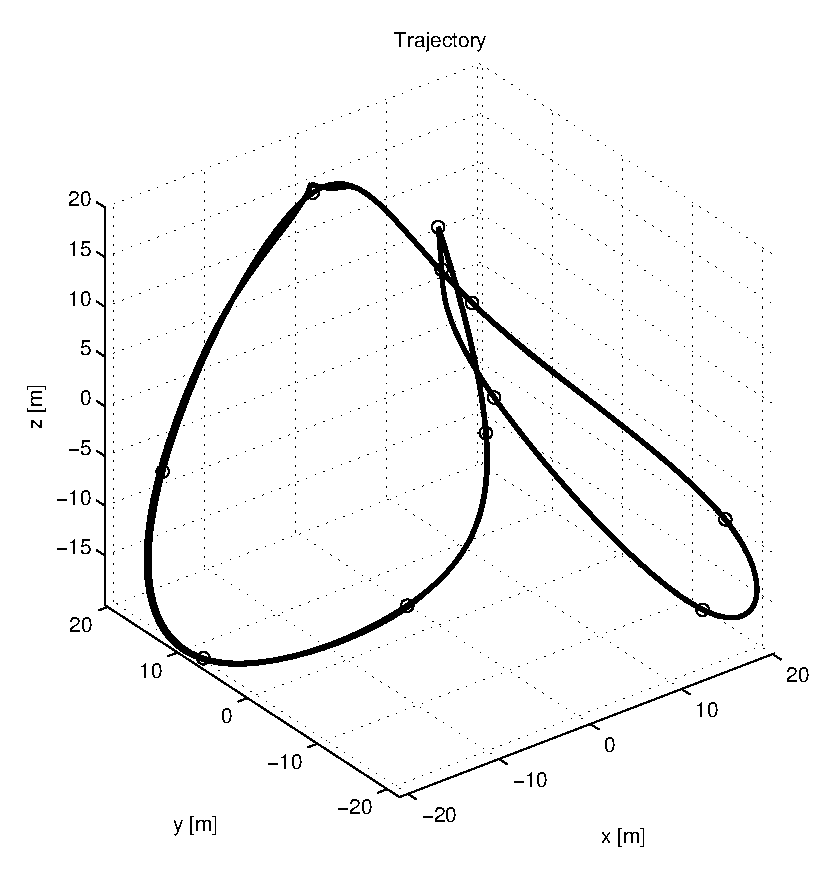
\includegraphics[width = \textwidth]{graphics/a}
  \end{minipage}
  \hfill
  \begin{minipage}[t]{0.48\textwidth}
%    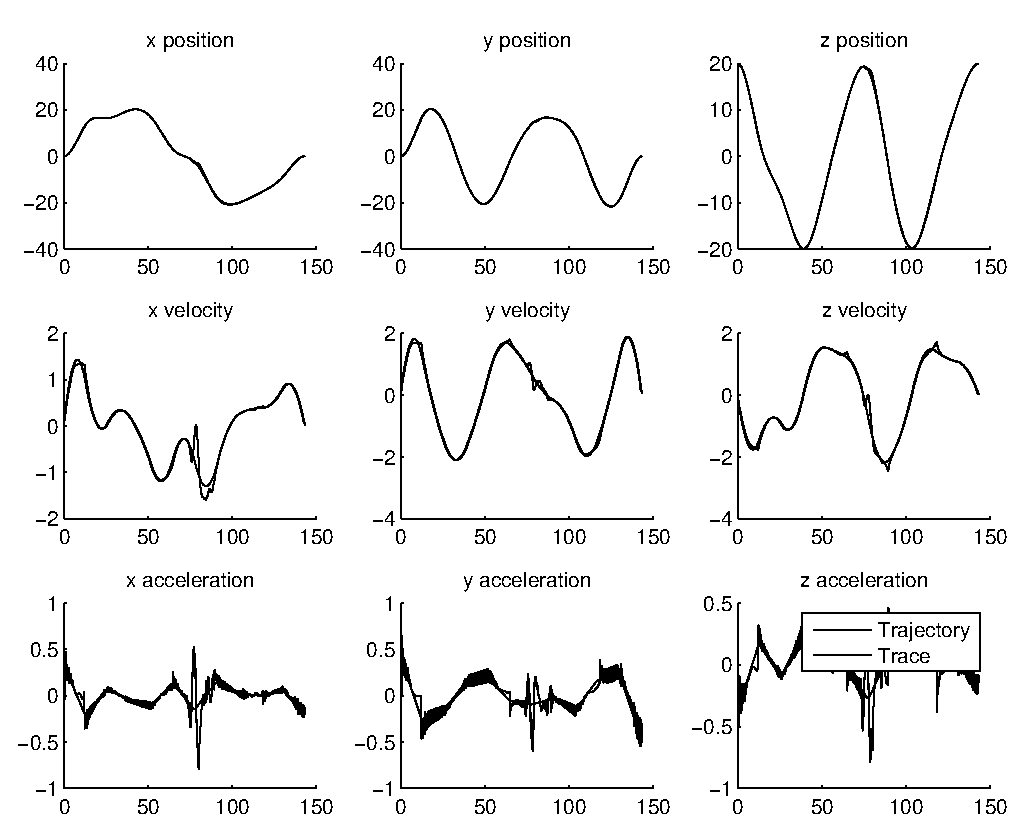
\includegraphics[width = \textwidth]{graphics/b.eps}
  \end{minipage}
  \caption{Trajectory following yields to extremly awesome tracking.}
  \label{fig:trajectoryfollowing}
\end{figure}



\subsection{Pure Pursuit Controller}
Another commonly used trajectory controller is Pure Pursuit \cite{snider}. To consider all dynamics of the trajectory, the reference intput is based on a lookahead point $\tilde{p}(t_{cl+\Delta T}) = \tilde{p}(t_{cl}) + \dot{\tilde{p}}(t_{cl})\Delta T + \ddot{\tilde{p}}(t_{cl}) + ORDNUNG$.
\subsection{Cross Track Error Controller}
see \cite{williams}

\section{Discussion}
\label{sec:discussion}

